\chapter{Evaluation}

In this chapter I will supply enough evidence about how the \ac{MA3C} algorithm learns faster and explores better than
\ac{A3C} in environments where subgoals can be defined.
All the code needed to make the following analysis was developed inside a project of the Universidad Pompeu Fabra researcher
Miquel Juyent.
The \ac{A3C} algorithm was fully provided by him while the algorithm \ac{MA3C} and the games Simple States and Complex
States have been developed by me.
% TODO PONER EL MONTEZUMA

\section{Simple States}

I have compared the performance of both algorithms \ac{A3C} (\ffref{alg:A3C}) and \ac{MA3C} (\ffref{alg:MA3C}) in Simple
States game (\ffref{subsec:SimpleStates}).

The hyperparameters used for both algorithms are:
\begin{itemize} % TODO PROGUNTAR A MIQUEL QUE FALTA
    \item The discount factor $\gamma = 0.99$.
    \item Batch size $20$. %TODO EXPLAIN
    \item The number of threads in which the algorithms have been parallelized is $8$.
    \item Subtrees $K = 3$. (just for \ac{MA3C})
    \item Entropy regularization term $\beta = 0.1$.
    \item Value regularization term $ = 0.5$ %TODO PONER EN EL ALGORITMO
\end{itemize}

This parameters have been chosen in order to show the disadvantages of \ac{A3C} as opposed to \ac{MA3C}.
There might be another combination of hyperparameters in which, at the end, both algorithms converge to the same solution.
Since the ultimate goal is to show how \ac{MA3C} explores better, this hyperparameters are good enough.

\begin{figure}[hbtp]
\begin{center}
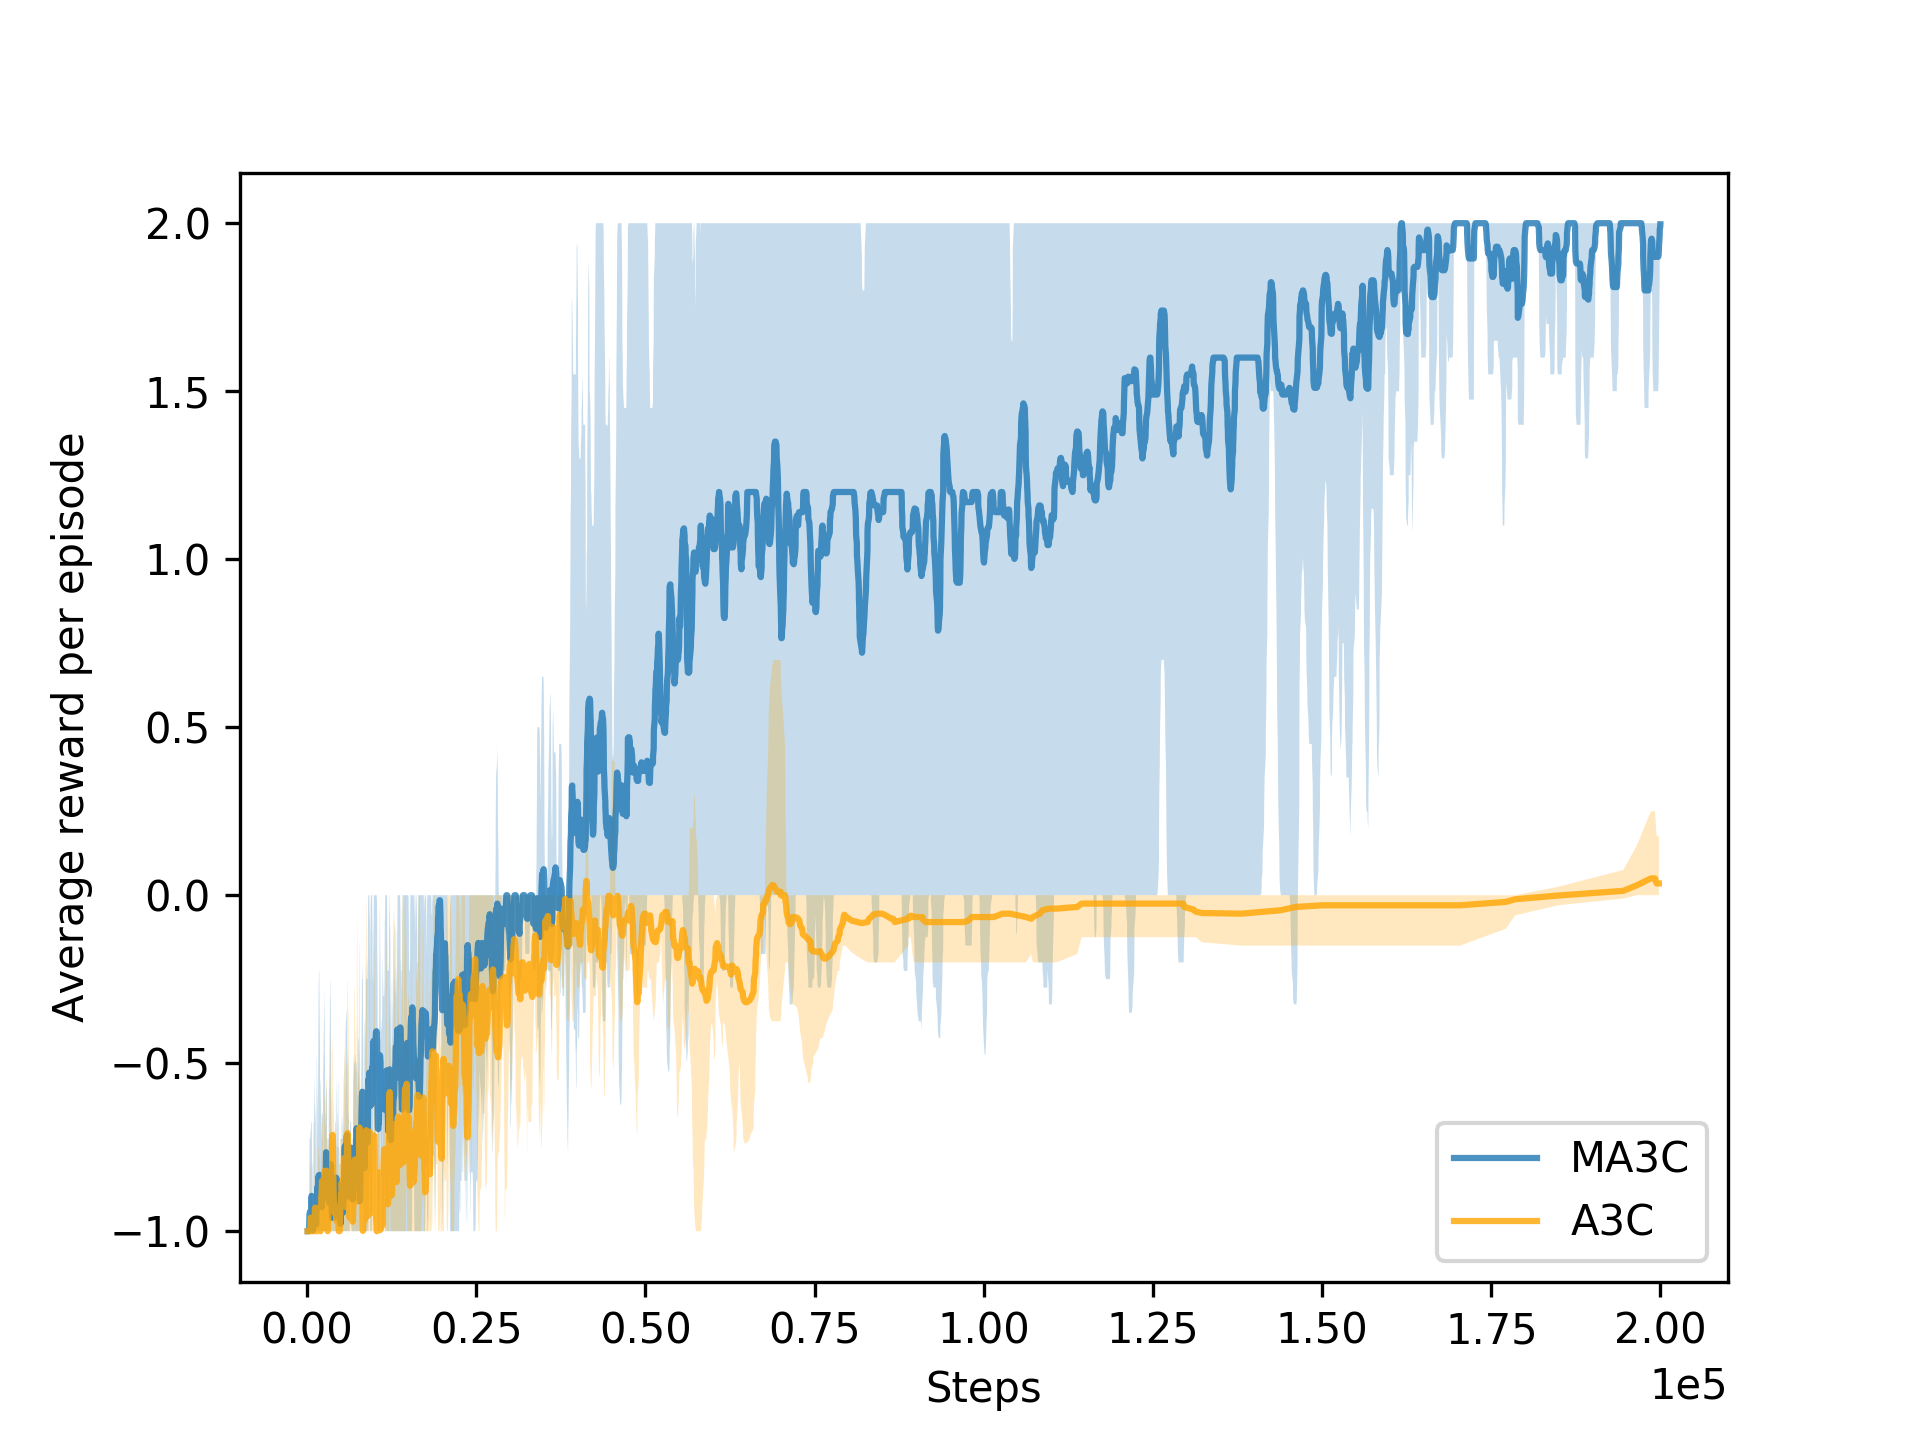
\includegraphics[width=250]{img/SimpleStates_performance.png}
\end{center}
\caption[Simple States performance]
{Average score over $5$ runs of \ac{A3C} and \ac{MA3C} algorithms in Simple States environment (200k steps/actions).
The shadow represents maximum and minimum values of those $5$ runs.
The graphics have been smoothed by a moving average with a $20$ steps window.}
\label{fig:SimpleStates_performance}
\end{figure}

The learning process of both algorithms measured by score over steps is shown in \ffref{fig:SimpleStates_performance}.
As you can see, \ac{MA3C} algorithm obtains score $2$ (checkpoint and door) while \ac{A3C} obtains score $0$ because it
reaches the checkpoint but then hits a wall.

This is due to the subtree changes which the algorithm makes every time it goes through any of the checkpoints (normal
and hidden).
Every time the change happens the data in the common network changes in a different manner (the direction of the gradient)
until it converges to common features for all subtrees.
Thanks to that the randomness is implicitly increased every time the change happens until convergence is achieved.
And, as far as more random actions lead to better exploration, this algorithm is using the subgoals (checkpoints) in
order to enhance exploration only when needed, specifically when a new phase is achieved.

It is important to remember that the hidden checkpoint does not give any reward, so in some cases there will be no need
of adding intermediate rewards, just subtree changes.
In general, when solving a problem with \ac{MA3C} it might be no need of doing reward shaping (\ffref{subsec:RewardShaping})
and carefully select the $\mathcal{F}$ function to ensure near-optimal policies.
The subtree changes can be done in any state and the optimal policies will remain the same, it will just enhance exploration
after reaching that states.

\section{Complex States}

\section{Montezuma's Revenge}
% TODO PONER EL NUMERO DE THREADS
% TODO WE OR I BUT NOT BOTH
%%% Local Variables: 
%%% mode: latex
%%% TeX-master: "../report"
%%% End: 